% Abbildung 2.4: Skalierungsgesetze nach Kaplan et al. (2020), schematisch (pgfplots)
\begin{tikzpicture}
  \begin{axis}[name=p1, width=0.36\linewidth, height=0.24\textheight, xmode=log, ymode=log,
    xlabel={Rechenaufwand [PF-Tage]}, ylabel={Test-Loss}, ymin=2, ymax=6, xmin=1e-8, xmax=1e1,
    ytick={2,3,4,5,6}, yticklabels={2,3,4,5,6}, minor ytick={2.5,3.5,4.5,5.5},
    title={\footnotesize $L = (C_{\min}/2{,}3\cdot 10^{8})^{-0{,}050}$}, title style={yshift=-3pt},
    tick label style={font=\scriptsize}, label style={font=\scriptsize}, grid=major, grid style={gray!25}]
    \addplot[blue!70!black, thick, domain=1e-8:1e1, samples=40] {(x/2.3e8)^(-0.050)};
  \end{axis}
  \begin{axis}[name=p2, at={(p1.east)}, anchor=west, xshift=0.9cm, width=0.36\linewidth, height=0.24\textheight,
    xmode=log, ymode=log, xlabel={Datensatzumfang [Tokens]}, ymin=2, ymax=6, xmin=1e7, xmax=1e10,
    ytick={2,3,4,5,6}, yticklabels={2,3,4,5,6}, minor ytick={2.5,3.5,4.5,5.5},
    title={\footnotesize $L = (D/5{,}4\cdot 10^{13})^{-0{,}095}$}, title style={yshift=-3pt},
    tick label style={font=\scriptsize}, label style={font=\scriptsize}, grid=major, grid style={gray!25}]
    \addplot[blue!70!black, thick, domain=1e7:1e10, samples=40] {(x/5.4e13)^(-0.095)};
  \end{axis}
  \begin{axis}[name=p3, at={(p2.east)}, anchor=west, xshift=0.9cm, width=0.36\linewidth, height=0.24\textheight,
    xmode=log, ymode=log, xlabel={Parameter ohne Embeddings}, ymin=2, ymax=6, xmin=1e5, xmax=1e9,
    ytick={2,3,4,5,6}, yticklabels={2,3,4,5,6}, minor ytick={2.5,3.5,4.5,5.5},
    title={\footnotesize $L = (N/8{,}8\cdot 10^{13})^{-0{,}076}$}, title style={yshift=-3pt},
    tick label style={font=\scriptsize}, label style={font=\scriptsize}, grid=major, grid style={gray!25}]
    \addplot[blue!70!black, thick, domain=1e5:1e9, samples=40] {(x/8.8e13)^(-0.076)};
  \end{axis}
\end{tikzpicture}
